\documentclass[4pt]{article}
\usepackage{spikey}
\usepackage{amsmath}
\usepackage{mathrsfs}
\usepackage{amssymb}
\usepackage{soul}
\usepackage{float}
\usepackage{graphicx}
\usepackage{hyperref}
\usepackage{fancyhdr}
\usepackage{xcolor}
\usepackage{chngcntr}
\usepackage{centernot}
\usepackage[shortlabels]{enumitem}
\usepackage[margin=1truein]{geometry}
\usepackage{tkz-graph}
\usepackage{dsfont}
\usepackage{caption}
\usepackage{subcaption}

\usepackage{setspace}
\linespread{0.75}

\geometry{margin=0.7cm, marginparwidth=1.1cm, marginparsep=0.1cm}

\counterwithin{equation}{section}
\counterwithin{figure}{section}

\begin{document}
	\section{Theory}
	\subsection{Information Entropy}
	\begin{definition}
		\textbf{Accuracy gain} from splitting $R$ into $R_1$ and $R_2$ based on loss $L(R)$:
		$
			L(R) - \frac{|R_1|L(R_1) + |R_2|L(R_2)}{|R_1| + |R_2|}
		$
	\end{definition}
	\begin{definition}
		Given a random variable $X \sim p$, the \textbf{entropy} measures the amount of randomness/uncertainty in an arbitrary realization of $X$. 
		\begin{align}
			H(X) &:= \mathbb{E}_{X \sim p}[- \log_2 p(X)]
		\end{align}
	\end{definition}
	\begin{definition}
		Given joint distribution $(X, Y) \sim p(X, Y)$, the \textbf{entropy of joint distribution} is defined as
		\begin{align}
			H(X, Y) := \mathbb{E}_{(X, Y) \sim p(X, Y)} [
			- \log_2 p(X, Y)
			] = - \sum_{x \in \mc{X}} \sum_{y \in \mc{Y}} p(x, y) \log_2 p(x, y)
		\end{align}
	\end{definition}
		\begin{definition}
		Given two random variables $X$ and $Y$, the \textbf{conditional entropy of $Y$ conditioned on specific realization of $X$} is defined to be 
		\begin{align}
			H(Y|X=x) := \mathbb{E}_{y \sim p(y|X=x)}[
				-\log_2 p(y|X=x)
			]
			= - \sum_{y \in \mc{Y}} p(y|X=x) \log_2 p(y|X=x)
		\end{align}
		The \textbf{expected conditional entropy}\footnote{This is independent of specific realization of $X$} is defined as 
		\begin{align}
			H(Y|X) = \mathbb{E}_{X \sim p(x)} [H(Y|X)]
			= \mathbb{E}_{X \sim p(x)} [\mathbb{E}_{y \sim p(y|X=x)}[
				-\log_2 p(y|X=x)]
			]
			= \sum_{x \in \mc{X}} p(x) H(Y|X=x) \\
			= - \sum_{x \in \mc{X}} p(x) \sum_{y \in Im(Y)} p(y|X=x) \log_2 p(y|X=x)
			= - \sum_{x \in \mc{X}} \sum_{y \in \mc{Y}} p(x, y) \log_2 p(y | X = x)
			= - \mathbb{E}_{(X, Y) \sim p(x, y)} [\log_2 p(Y|X)]
		\end{align}
	\end{definition}
	\begin{proposition}
		For every $X \in \Delta(\mc{X})$, $H(X) \geq 0$.
	\end{proposition}
	\begin{proposition}[Chain Rule]
		$
			H(X, Y)=H(X | Y)+H(Y)=H(Y | X)+H(X)
		$
	\end{proposition}
	\begin{proposition}
		If $X \perp Y$, then knowing $X$ does not provide extra information (i.e. reduce entropy) of $Y$. That is $H(Y|X) = H(Y)$.
	\end{proposition}
	\begin{proposition}
		$Y$ becomes deterministic by knowing $Y$, that is, $H(Y|Y) = 0$.
	\end{proposition}
	\begin{proposition}
		By knowing $X$, the uncertainty about $Y$ is reduced: $H(Y|X) \leq H(Y)$.
	\end{proposition}
	\begin{definition}
		The \textbf{information gain} in $Y$ due to $X$, or \textbf{mutual information} of $X$ and $Y$ is defined to be
		\begin{align}
			IG(Y|X) &:= H(Y) - H(Y|X)
		\end{align}
		When $X$ is completely uninformative about $Y$: $H(Y|X) = H(Y)$, then $IG(Y|X) = 0$.\\
		When $X$ is completely information about $Y$: $H(Y|X) = 0$ (deterministic), then $IG(Y|X) = H(Y)$.
	\end{definition}
	\begin{proposition}[Symmetry of Information Gain]
		\begin{align}
			IG(Y|X) := H(Y) - H(Y|X)
			= H(X, Y) - H(X|Y) - H(Y|X) \\
			= H(Y|X) + H(X) - H(X|Y) - H(Y|X)
			= H(X) - H(X|Y) 
			= IG(X|Y)
		\end{align}
	\end{proposition}
	\paragraph{BVD: Deterministic} 
	\begin{align}
		\red{\mathbb{E}_{x, \mathcal{D}}\left[\left(h_{\mathcal{D}}(x)-f(x)\right)^{2}\right]=\mathbb{E}_{x, \mathcal{D}}\left[\left(h_{\mathcal{D}}(x)-\mathbb{E}_{\mathcal{D}}\left[h_{\mathcal{D}}(x) | x\right]\right)^{2}\right]+\mathbb{E}_{x}\left[\left(\mathbb{E}_{\mathcal{D}}\left[h_{\mathcal{D}}(x) | x\right]-f(x)\right)^{2}\right]}
	\end{align}
	\paragraph{BVD: Stochastic}Let $(\vex\upi, y\upi) \in \mc{X} \times \R$ denote one training instance such that
	$
		(\vex\upi, y\upi) \overset{i.i.d.}{\sim} p_{\tx{sample}}
	$
	,where $p_{\tx{sample}} \in \Delta (\mc{X} \times \R)$. \\
	Fixing $N \in \N$, one can construct a new distribution $p_{\tx{dataset}} \in \Delta (\mc{X} \times \R)^N$ such that 
	$
		(\vex\upi, y\upi)_{i=1}^N =: \mc{D} \sim p_{\tx{dataset}}
	$
	Given a (random) training set $\mc{D}$, a (random) classifier function $h_{\mc{D}} \in \mc{H}$ is generated. \\
	For every \emph{query point} $\vex \in \mc{X}$, the prediction $h_\mc{D}(\vex)$ is therefore random. \\
	Suppose $y$ is not deterministic in $x$, then the expected mean squared error when the model is applied on new instances sampled from $p_{\tx{sample}}$ is
	\begin{align}
		\mathbb{E}_{\vex, y, \mc{D}}[(h_\mc{D}(\vex) - y)^2] &= \mathbb{E}_{\mc{D}}[
		\mathbb{E}_{\vex, y} [(h_\mc{D}(\vex) - y)^2|\mc{D}]
		]
		= \mathbb{E}_{\mc{D}}[
		\mathbb{E}_{\vex, y} [(h_\mc{D}(\vex) - \mathbb{E}_y[y|x] + \mathbb{E}_y[y|x] - y)^2|\mc{D}]
		]\\ 
		&= \mathbb{E}_{\mc{D}} \{
		\mathbb{E}_x[
		\mathbb{E}_y[
		(h_\mc{D}(\vex) - \mathbb{E}_y[y|x])^2
		]
		]
		+ 2 \mathbb{E}_{x,y}[(h_\mc{D}(\vex) - \mathbb{E}_y[y|x]) (\mathbb{E}_y[y|x] - y)] 
		+ \mathbb{E}_{x, y} (\mathbb{E}_y[y|x] - y)^2
		\}\\
		&= \mathbb{E}_{\mc{D}} \{
		\mathbb{E}_x[
		(h_\mc{D}(\vex) - \mathbb{E}_y[y|x])^2
		]
		+ 2 \mathbb{E}_{x,y}[(h_\mc{D}(\vex) - \mathbb{E}_y[y|x]) (\mathbb{E}_y[y|x] - y)] 
		+ \mathbb{E}_{x, y} [(\mathbb{E}_y[y|x] - y)^2]
		\} \\
	\end{align}
	By law of iterative expectation,
	\begin{align}
		\mathbb{E}_{x,y}[(h_\mc{D}(\vex) - \mathbb{E}_y[y|x]) (\mathbb{E}_y[y|x] - y)] &= \mathbb{E}_x [
		\mathbb{E}_y[
		(h_\mc{D}(\vex) - \mathbb{E}_y[y|x]) (\mathbb{E}_y[y|x] - y)
		]]
		= \mathbb{E}_x[
		(h_\mc{D}(\vex) - \mathbb{E}_y[y|x]) (\mathbb{E}_y[y|x] - \mathbb{E}_y[y])
		]
		= 0
	\end{align}
	By dropping irrelevant expectation operators, 
	\begin{align}
		\Delta &= \mathbb{E}_\mc{D}[\mathbb{E}_x[(h_\mc{D}(\vex) - \mathbb{E}_y[y|x])^2]] + \underbrace{\mathbb{E}_{x, y}[(\mathbb{E}_y[y|x] - y)^2]}_{\tx{Bayes Error } \varepsilon^2}
		= \mathbb{E}_\mc{D}[\mathbb{E}_x[
		(h_\mc{D}(\vex) - \mathbb{E}_y[y|x])^2
		]] + \varepsilon^2 \\
		&= \mathbb{E}_\mc{D}[\mathbb{E}_x[
		(h_\mc{D}(\vex) - \mathbb{E}_\mc{D}[h_\mc{D}(x)|x] + \mathbb{E}_\mc{D}[h_\mc{D}(x)|x] -  \mathbb{E}_y[y|x])^2
		]] + \varepsilon^2
	\end{align}
	Note that
	$
		\mathbb{E}_\mc{D}[
		\mathbb{E}_x[
		(h_\mc{D}(\vex) - \mathbb{E}_\mc{D}[h_\mc{D}(x)|x])
		(\mathbb{E}_\mc{D}[h_\mc{D}(x)|x] -  \mathbb{E}_y[y|x])
		]] = 0
	$
	The first component reduced to zero after applying law of iterative expectation. \ul{Non-deterministic case}
	\begin{align}
		\red{\mathbb{E}_{x, y, \mathcal{D}}\left[\left(h_{\mathcal{D}}(x)-y\right)^{2}\right]=\mathbb{E}_{x, \mathcal{D}}\left[\left(h_{\mathcal{D}}(x)-\mathbb{E}_{\mathcal{D}}\left[h_{\mathcal{D}}(x) | x\right]\right)^{2}\right]+\mathbb{E}_{x}\left[\left(\mathbb{E}_{\mathcal{D}}\left[h_{\mathcal{D}}(x) | x\right]-\mathbb{E}_{y}[y | x]\right)^{2}\right]+\mathbb{E}_{x, y}\left[\left(\mathbb{E}_{y}[y | x]-y\right)^{2}\right]}
	\end{align}
	
	\section{Mathematics \& Probability}
	$p(x | \mu, \Sigma)=\frac{1}{(2 \pi)^{d / 2} \operatorname{det}(\Sigma)^{1 / 2}} \exp \left\{-\frac{1}{2}(x-\mu)^{T} \Sigma^{-1}(x-\mu)\right\}$ \\
	$\operatorname{Var}(X)=\mathbb{E}\left[(X-\mu)(X-\mu)^{T}\right] \in \mathbb{R}^{d \times d}$ \\
	$\operatorname{Cov}(X, Y)=\mathbb{E}\left[\left(X-\mu_{X}\right)\left(Y-\mu_{y}\right)^{T}\right] \in \mathbb{R}^{d \times d}$ \quad $p(\theta | \text { data })=\frac{p(\text { data } | \theta) p(\theta)}{p(\text { data })}$ \quad $\theta^{\mathrm{MAP}}=\underset{\theta}{\operatorname{argmax}} p(\theta | \text { data })=\underset{\theta}{\operatorname{argmax}} p(\operatorname{data} | \theta) p(\theta)$ \\
	$\begin{aligned}\theta^{\mathrm{MAP}} &=\underset{\theta}{\operatorname{argmax}} p\left(X_{1}, \ldots, X_{N} | \theta\right) p(\theta)=\underset{\theta}{\operatorname{argmax}} p(\theta) \prod_{i=1}^{N} p\left(X_{i} | \theta\right) =\underset{\theta}{\operatorname{argmax}} \log p(\theta)+\sum_{i=1}^{N} \log p\left(X_{i} | \theta\right) \end{aligned}$
	\begin{proposition}[Law of Total Expectation]
	$\mathbb{E}_Y [\mathbb{E}_{X|Y}[X|Y]] = \expect{X}$.
		\begin{proof}
			$\mathbb{E}[\mathbb{E}[X | Y]]=\int\left[\int x p(x | y) d x\right] p(y) d y=\iint x p(x, y) d x d y=\mathbb{E}[X]$
		\end{proof}
	\end{proposition}
	$\underset{\mathbf{w}}{\operatorname{minimize}} \mathcal{J}(\mathbf{w})=: \frac{1}{2}\|\mathbf{t}-\mathbf{X} \mathbf{w}\|_{2}^{2}$ \quad $\mathcal{J}(\mathbf{w})=\frac{1}{2}\|\mathbf{t}\|_{2}^{2}+\frac{1}{2} \mathbf{w}^{\top} \mathbf{X}^{\top} \mathbf{X} \mathbf{w}-\mathbf{t}^{\top} \mathbf{X} \mathbf{w}$. \\
	\begin{theorem}[Bayes Optimal]
		$
			\argmin_{y} \expect{(y-t)^2|\vex} = \expect{t|\vex}
		$
		where $t \sim p(t|\vex)$.
	\end{theorem}
	\textbf{Multi-class Classification} $\vez = \bf{W} \vex + \veb$ (aka \emph{logits}) Input dim = $D$, output dim = $K$, $\textbf{W} \in \R^{K \times D}$ \\
	Pred\_prob:$y_{k}=\operatorname{softmax}\left(z_{1}, \ldots, z_{K}\right)_{k}=\frac{e^{z_{k}}}{\sum_{k^{\prime}} e^{z_{k^{\prime}}}}$ \quad
	$\mathcal{L}_{\mathrm{CE}}(\mathbf{y}, \mathbf{t})=-\sum_{k=1}^{K} t_{k} \log y_{k} = - \textbf{t}^T (\log (y))$ (\emph{Softmax-cross-entropy}). \\
	\begin{align*}
		\begin{aligned} \frac{\partial \mathcal{L}_{\mathrm{CE}}}{\partial \mathbf{w}_{k}} =\frac{\partial \mathcal{L}_{\mathrm{CE}}}{\partial z_{k}} \cdot \frac{\partial z_{k}}{\mathbf{w}_{k}}=\left(y_{k}-t_{k}\right) \cdot \mathbf{x}, 
		\quad \mathbf{w}_{k}  \leftarrow \mathbf{w}_{k}-\alpha \frac{1}{N} \sum_{i=1}^{N}\left(y_{k}^{(i)}-t_{k}^{(i)}\right) \mathbf{x}^{(i)} \end{aligned},
		\quad \textbf{W} \leftarrow \textbf{W} - \frac{\alpha}{N} (\vey - \textbf{t}) \textbf{X}
	\end{align*}
	
	\begin{minipage}[t]{.15\linewidth}
		\begin{align*}
			\tx{(Forward)} \\
			\begin{array}{l}{\mathbf{z}=\mathbf{W}^{(1)} \mathbf{x}+\mathbf{b}^{(1)}} \\ {\mathbf{h}=\sigma(\mathbf{z})} \\ {\mathbf{y}=\mathbf{W}^{(2)} \mathbf{h}+\mathbf{b}^{(2)}} \\ {\mathcal{L}=\frac{1}{2}\|\mathbf{t}-\mathbf{y}\|^{2}}\end{array}
		\end{align*}
	\end{minipage}
	\begin{minipage}[t]{.15\linewidth}
		\begin{align*}
			\tx{(Backward)} \\
			\begin{aligned} \overline{\mathcal{L}} &=1 \\ \overline{\mathbf{y}} &=\overline{\mathcal{L}}(\mathbf{y}-\mathbf{t}) \\ \overline{\mathbf{W}^{(2)}} &=\overline{\mathbf{y}} \mathbf{h}^{\top} \\ \overline{\mathbf{h}^{(2)}} &=\overline{\mathbf{y}} \\ \overline{\mathbf{h}} &=\mathbf{W}^{(2) \top} \overline{\mathbf{y}} \\ \overline{\mathbf{z}} &=\overline{\mathbf{h}} \circ \sigma^{\prime}(\mathbf{z}) \\ \overline{\mathbf{W}^{(1)}} &=\overline{\mathbf{z}} \mathbf{x}^{\top} \\ \overline{\mathbf{b}^{(1)}} &=\overline{\mathbf{z}} \end{aligned}
		\end{align*}
	\end{minipage}
	\vline
	\begin{minipage}[t]{.15\linewidth}
	  	\begin{align*}
	  		\tx{(Forward: Reg)} \\
			\begin{aligned} z &=w x+b \\ y &=\sigma(z) \\ \mathcal{L} &=\frac{1}{2}(y-t)^{2} \\ \mathcal{R} &=\frac{1}{2} w^{2} \\ \mathcal{L}_{\mathrm{reg}} &=\mathcal{L}+\lambda \mathcal{R} \end{aligned}
		\end{align*}
	\end{minipage}
	\begin{minipage}[t]{.15\linewidth}
	\begin{align*}
		\tx{(Backward I)} \\
		\begin{aligned} \overline{\mathcal{L}_{\text {reg }}} &=1 \\ \overline{\mathcal{R}} &=\overline{\mathcal{L}_{\text {reg }}} \frac{\mathrm{d} \mathcal{L}_{\text {reg }}}{\mathrm{d} \mathcal{R}} \\ &=\overline{\mathcal{L}_{\text {reg }}} \lambda \\ \overline{\mathcal{L}} &=\overline{\mathcal{L}_{\text {reg }}} \frac{\mathrm{d} \mathcal{L}_{\text {reg }}}{\mathrm{d} \mathcal{L}} \\ &=\overline{\mathcal{L}_{\text {reg }}} \\ \bar{y} &=\overline{\mathcal{L}} \frac{\mathrm{d} \mathcal{L}}{\mathrm{d} y} \\ &=\overline{\mathcal{L}}(y-t)
		\end{aligned}
	\end{align*}
	\end{minipage}
	\begin{minipage}[t]{0.15\linewidth}
		\begin{align*}
			\tx{(Backward II)} \\
			\begin{aligned} \bar{z} &=\bar{y} \frac{\mathrm{d} y}{\mathrm{d} z} \\ &=\bar{y} \sigma^{\prime}(z) \\ \bar{w} &=\bar{z} \frac{\partial z}{\partial w}+\overline{\mathcal{R}} \frac{\mathrm{d} \mathcal{R}}{\mathrm{d} w} \\ &=\bar{z} x+\overline{\mathcal{R}} w \\ \bar{b} &=\bar{z} \frac{\partial z}{\partial b} \\ &=\bar{z} \end{aligned}
		\end{align*}
	\end{minipage}
	\vline
	\begin{minipage}[t]{0.15\linewidth}
		\begin{align*}
			\mathbf{g}_{i}=\nabla \mathcal{L}\left(\mathbf{w}, \mathbf{x}_{i}, t_{i}\right) \\
			\tx{(GD)} \\
			\mathbf{w} \leftarrow \mathbf{w}-\eta \sum_{i=1}^{N} g_{i} \\
			\tx{(SGD)} \\
			i \sim \mathcal{U}[1, N], \\
			\mathbf{w} \leftarrow \mathbf{w}-\eta g_{i} \\
			\tx{(mSGD)} \\
			M \subset\{1, \ldots, N\}, \\
			\mathbf{w} \leftarrow \mathbf{w}-\eta \sum_{i \in M}^{|M|} g_{i}
		\end{align*}
	\end{minipage}
	\section{Misc}
	\begin{enumerate}
		\item Activation functions $\tanh (z)=\frac{\exp (z)-\exp (-z)}{\exp (z)+\exp (-z)}$ \quad $\sigma(z)=\frac{1}{1+\exp (-z)}$ \quad $\operatorname{ReLU}(z)=\max (0, z)$.
		\item \textbf{Parametric} \ul{Benefits} (i) Simpler (interpretability) (ii) Speed (iii) Less Data; 
		\\ \ul{Drawbacks} (i) Constrained (ii) Limited Complexity (iii) Poor fit.
		\item \textbf{Non-parametric} \ul{Benefits} (i) Flexibility (ii) Power (No prior assumptions) (iii) Performance;
		\\ \ul{Drawbacks} (i) More data (ii) Slower (iii) Overfitting.
		\item Decision of linear models: $\textbf{W} \cdot \vex + \veb = \textbf{0}$ (hyperplane).
	\end{enumerate}
	\begin{minipage}[t]{0.3\linewidth}
		\textbf{SVM}
		\begin{align*}
			\begin{aligned} \text {0-1 loss: } & \mathcal{L}_{0-1}(z, t)=\mathbb{I}\{\operatorname{sign}(z) \neq t\} \\ \text { Hinge loss: } & \mathcal{L}_{\mathrm{H}}(z, t)=\max \{0,1-z t\} \end{aligned} \\
			\min _{\mathbf{w}, b} \Sigma_{i=1}^{N} \max \left\{0,1-t^{(i)} z^{(i)}(\mathbf{w}, b)\right\} \\
			\min _{\mathbf{w}, b} \Sigma_{i=1}^{N} \max \left\{0,1-t^{(i)} z^{(i)}(\mathbf{w}, b)\right\}+\frac{\lambda}{2}\|\mathbf{w}\|_{2}^{2}
		\end{align*}
		\par Optimize: gradient descent.
%		\centering
%		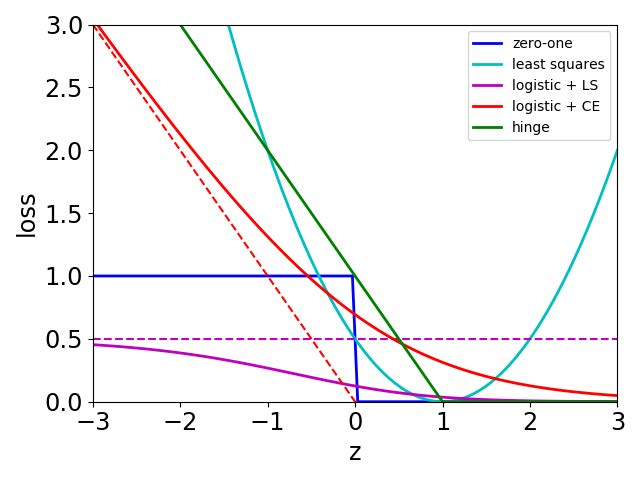
\includegraphics[width=0.5\linewidth]{loss.jpg}
	\end{minipage}
	\vline
	\begin{minipage}[t]{0.3\linewidth}
		\textbf{Boosting} \\
		\par Weighted training set: we can learn a classier using different costs (aka weights) for examples.
		\begin{align*}
			\Sigma_{n=1}^{N} w^{(n)} \mathbb{I}[h(x^{(n)}) \neq t^{(n)}] \\
			w^(n) > 0 \land \Sigma_{n=1}^{N} w^{(n)}=1
		\end{align*}
		\par \textbf{Decision Stump} A decision tree with a single split. \\
		AdaBoost \textbf{reduces bias} by making each classier focus on previous mistakes.
	\end{minipage}
\end{document}









